\documentclass[tikz, border=10pt]{standalone}
\usepackage{pgfplots}
\usepgfplotslibrary{groupplots}
\pgfplotsset{compat=1.18}

\begin{document}
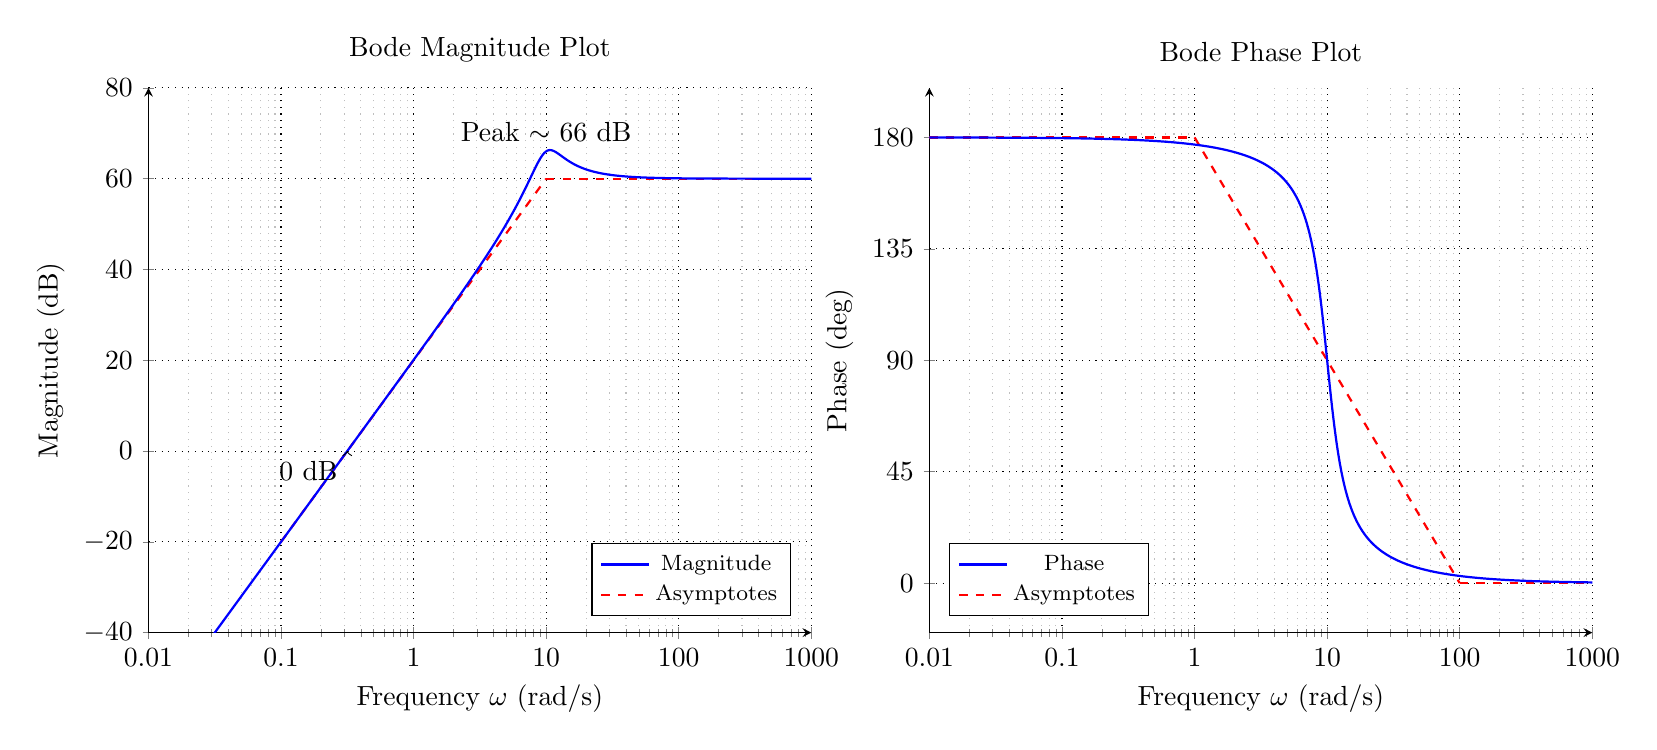
\begin{tikzpicture}
    \begin{groupplot}[
        group style={
            group size=2 by 1,
            horizontal sep=1.5cm,
        },
        width=10cm, height=8.5cm,
        xlabel={Frequency $\omega$ (rad/s)},
        xmin=0.01, xmax=1000,
        xmode=log,
        grid=both,
        major grid style={dotted, black},
        minor grid style={dotted, gray!50},
        axis lines=left,
        xtick={0.01, 0.1, 1, 10, 100, 1000},
        xticklabels={$0.01$, $0.1$, $1$, $10$, $100$, $1000$},
    ]

    % Magnitude Plot
    \nextgroupplot[
        ylabel={Magnitude (dB)},
        ymin=-40, ymax=80,
        legend pos=south east,
        legend style={font=\footnotesize},
        title={Bode Magnitude Plot}
    ]
    % Asymptotes Magnitude
    % H(s) ~ 10s^2 for w < 10. w=0.1 -> -20 dB. w=1 -> 20 dB. w=10 -> 60 dB.
    \draw[thick, red, dashed] (axis cs: 0.1, -20) -- (axis cs: 10, 60);
    % w > 10: Constant 60 dB.
    \draw[thick, red, dashed] (axis cs: 10, 60) -- (axis cs: 1000, 60);
    
    % Actual Curve
    % |H(jw)| = 1000w^2 / sqrt((100-w^2)^2 + (5w)^2)
    \addplot[thick, blue, domain=0.01:1000, samples=500] {20*log10( 1000*x^2 / sqrt( (100-x^2)^2 + (5*x)^2 ) )};
    
    \addlegendentry{Magnitude}
    \addlegendimage{thick, red, dashed}
    \addlegendentry{Asymptotes}

    % Annotations
    \node[anchor=north east] (p1) at (axis cs: 0.316, 0) {0 dB};
    \draw[->] (p1) -- (axis cs: 0.316, 0);
    \node[anchor=south] at (axis cs: 10, 66) {Peak $\sim$ 66 dB};

    % Phase Plot
    \nextgroupplot[
        ylabel={Phase (deg)},
        ymin=-20, ymax=200,
        ytick={0, 45, 90, 135, 180},
        legend pos=south west,
        legend style={font=\footnotesize},
        title={Bode Phase Plot}
    ]
    
    % Asymptotes Phase
    % Constant 180 for double zero
    % Double pole at 10: 180 (w<1) -> 90 (at w=10) -> 0 (w>100)
    \draw[thick, red, dashed] (axis cs: 0.01, 180) -- (axis cs: 1, 180);
    \draw[thick, red, dashed] (axis cs: 1, 180) -- (axis cs: 100, 0);
    \draw[thick, red, dashed] (axis cs: 100, 0) -- (axis cs: 1000, 0);

    % Actual Curve Phase
    % Phi = 180 - atan2( 5w, 100-w^2 )
    \addplot[thick, blue, domain=0.01:1000, samples=500] {180 - atan2(5*x, 100-x^2)};

    \addlegendentry{Phase}
    \addlegendimage{thick, red, dashed}
    \addlegendentry{Asymptotes}

    \end{groupplot}
\end{tikzpicture}
\end{document}
